




\begin{center}
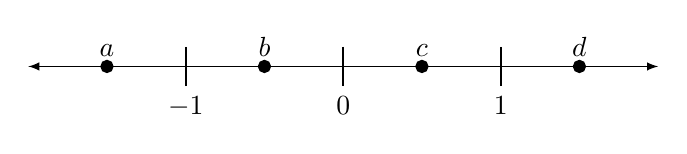
\begin{tikzpicture}
\draw[>=latex,<->](0,0)--(8,0);
    \draw[thick, fill=black] (2,.25)--(2,-.25) node[below]{$-1$};
    \draw[thick, fill=black] (4,.25)--(4,-.25) node[below]{$0$};
    \draw[thick, fill=black] (6,.25)--(6,-.25) node[below]{$1$};

    \draw[thick, fill=black] (1,0) circle (.07cm) node[above]{$a$};
    \draw[thick, fill=black] (3,0) circle (.07cm) node[above]{$b$};
    \draw[thick, fill=black] (5,0) circle (.07cm) node[above]{$c$};
     \draw[thick, fill=black] (7,0) circle (.07cm) node[above]{$d$};
\end{tikzpicture}
\end{center}


   Which of the following has the greatest value?


\ifsat
	\begin{enumerate}[label=\Alph*)]
		\item   $a+b$
		\item  $c+d$
		\item  $a-d$
		\item  $d-a$%
	\end{enumerate}
\else
\fi

\ifacteven
	\begin{enumerate}[label=\textbf{\Alph*.},itemsep=\fill,align=left]
		\setcounter{enumii}{5}
		\item   $a+b$
		\item  $b+c$
		\item  $c+d$
		\addtocounter{enumii}{1}
		\item  $a-d$
		\item  $d-a$%
	\end{enumerate}
\else
\fi

\ifactodd
	\begin{enumerate}[label=\textbf{\Alph*.},itemsep=\fill,align=left]
		\item   $a+b$
		\item  $b+c$
		\item  $c+d$
		\item  $a-d$
		\item  $d-a$%
	\end{enumerate}
\else
\fi

\ifgridin
  $d-a$%

\else
\fi

